\documentclass[a4paper,12pt]{article}
%添加宏包
\usepackage{titlesec,titletoc}
\usepackage{graphicx}%用于图像
\usepackage{times}
\usepackage{fontspec,xunicode,xltxtra}%XeLaTeX相关字体库,系统字库
\usepackage{multicol} %分栏
\usepackage{balance}%双栏文档底部对齐
%\usepackage{tocvsec2}
\usepackage{indentfirst}             % 首行缩进
\usepackage{setspace}                % 调节行间距
\usepackage{booktabs}                % 用于表格中加下划线
\usepackage{fancyhdr}                % 页眉页脚
\usepackage{type1cm}                 % 控制字体大小
\usepackage{amsmath}				%数学公式
\usepackage{amssymb}				%漂亮的数学公式排版
\usepackage{textcomp} 
\usepackage{multirow}
%\usepackage{bbding}                  % 一些特殊符号
%\usepackage{mathrsfs}
%\usepackage{amsthm}
\usepackage{amstext}
%\usepackage{makeidx}                 % 建立索引
\usepackage{float}
%\usepackage{bm}
\iffalse
\usepackage[a4paper,left=1.5cm,right=1.5cm, 
top=2.5cm,bottom=2cm,textwidth=14cm,textheight=20.3cm,
includehead,headheight=15pt,headsep=25pt]{geometry}
\fi

%页面布局
\usepackage{geometry} 
\geometry{paperwidth=21cm,paperheight=29.5cm}
\geometry{textwidth=17cm,lines=26} 
\geometry{left=2cm,right=2cm, top=1.5cm,bottom=2cm} 
\geometry{includehead,headheight=5pt,headsep=15pt}

%字体字号重定义(方便快捷使用)
\newcommand{\wuhao}{\fontsize{10.5pt}{20pt}\selectfont}%五号字体,20磅行距
\newcommand{\xiaosan}{\fontsize{15pt}{22pt}\selectfont}%小三字体,1.5倍行距
\newcommand{\numshihao}{\fontsize{10pt}{20pt}\selectfont}%10号字体,20磅行距
\newcommand{\erhao}{\fontsize{22pt}{22pt}\selectfont}%二号字体,单倍行距
\newcommand{\yemeiyejiao}{\fontsize{12pt}{12pt}\selectfont}%页眉页脚字号

%\sectionfont{\kai\selectfont}%节标题字体
%\subsectionfont{\kai}%	 小节标题字体
%\subsubsectionfont{\kai}	% 小小节标题字体
%\newcommand\chfrac[2]{\frac{\;#1\;}{\;#2\;}}%分数线

%中文字体设置
\XeTeXlinebreaklocale "zh"
\XeTeXlinebreakskip = 0pt plus 1pt minus 0.1pt%自动断行
\setmainfont[BoldFont={SimHei},ItalicFont={KaiTi}]{SimSun}%设置默认字体
\setsansfont{SimHei}
\setmonofont{SimSun}
\newfontfamily\song{SimSun.ttc}%宋体
\newfontfamily\hei{SimHei.ttf}%黑体
\newfontfamily\roman{Times New Roman}


%命令重定义自定义
%\newtheorem{theorem}{定理}
%\newtheorem{definition}{定义}
%\newtheorem{property}{问题}
%\newtheorem{proposition}{猜测}
%\newtheorem{lemma}{引理}
%\newtheorem{corollary}{推论}
%\renewcommand{\contentsname}{\center\hei{\sanhao{目录}}}
\renewcommand{\refname}{\textbf{\normalsize{参考文献}}}      % 将References改为参考文献、
\renewcommand{\figurename}{\song 图}
\renewcommand{\tablename}{\song 表}


\titleformat{section}[形状]{格式}{标题序号}{序号与标题间距}{标题前命令}[标题后命令]

%封面
\title{\erhao{\textbf{毕设翻译}}}
\author{\song\wuhao{赵欣}}
\date{\song\wuhao{2014年5月3日}}

%定义页眉页脚
\pagestyle{fancy}
\lhead{}
\chead{\song\yemeiyejiao{全环面CVT的多目标几何优化}}
\rhead{}
\lfoot{}
\cfoot{}
\rfoot{}

\iffalse
%图片定义
\makeatletter
\def\@captype{figure}
\newcommand\figurecaption{\def\@captype{figure}\caption}
\newcommand\tablecaption{\def\@captype{table}\caption}
\makeatother
\fi

\begin{document}
\centering
\maketitle
\thispagestyle{empty}
%%%
%% This is file `balance.sty',
%% generated with the docstrip utility.
%%
%% The original source files were:
%%
%% balance.dtx  (with options: `package')
%% =============================================
%% IMPORTANT NOTICE:
%% 
%% This program can be redistributed and/or modified under the terms
%% of the LaTeX Project Public License Distributed from CTAN
%% archives in directory macros/latex/base/lppl.txt; either
%% version 1 of the License, or any later version.
%% 
%% This is a generated file.
%% It may not be distributed without the original source file balance.dtx.
%% 
%% Full documentation can be obtained by LaTeXing that original file.
%% Only a few abbreviated comments remain here to describe the usage.
%% =============================================
%% Copyright 1993-1999 Patrick W Daly
%% Max-Planck-Institut f\"ur Aeronomie
%% Max-Planck-Str. 2
%% D-37191 Katlenburg-Lindau
%% Germany
%% E-mail: daly@linmpi.mpg.de
\NeedsTeXFormat{LaTeX2e}[1994/06/01]
\ProvidesPackage{balance}
         [1999/02/23 4.3 (PWD)]
 % In order to balance the columns on a page, \balance must be given
 % somewhere within the first column. To turn off the feature, give
 % \nobalance. One has to look at the unbalanced text first to decide
 % where best to place \balance.
 %-----------------------------------------------------------
\newcommand{\@BAlancecol}{\if@twocolumn
  \setbox0=\vbox{\unvbox\@outputbox} \@tempdima=\ht0
  \advance\@tempdima by \topskip \advance\@tempdima
     by -\baselineskip \divide\@tempdima by 2
     \splittopskip=\topskip
  {\vbadness=\@M \loop \global\setbox3=\copy0
   \global\setbox1=\vsplit3 to \@tempdima
   \ifdim\ht3>\@tempdima \global\advance\@tempdima by 1pt \repeat}
   \setbox\@leftcolumn=\vbox to \@tempdima{\unvbox1\vfil}
   \setbox\@outputbox=\vbox to \@tempdima
     {\dimen2=\dp3\unvbox3\kern-\dimen2
      \vfil}
  \fi}
\newif\if@BAlanceone
\global\@BAlanceonefalse
\newdimen\oldvsize
\newcommand{\@BAdblcol}{\if@firstcolumn
       \unvbox\@outputbox \penalty\outputpenalty
       \global\oldvsize=\@colht \global\multiply \@colht by 2
       \global\@BAlanceonetrue
       \global\@firstcolumnfalse
  \else \global\@firstcolumntrue
       \if@BAlanceone
       \global\@BAlanceonefalse\@BAlancecol
       \global\@colht=\oldvsize \else
       \PackageWarningNoLine{balance}
          {You have called \protect\balance\space
             in second column\MessageBreak
           Columns might not be balanced}\fi
     \setbox\@outputbox\vbox to \@colht{\hbox to\textwidth
     {\hbox to\columnwidth {\box\@leftcolumn \hss}\hfil
      \vrule width\columnseprule\hfil \hbox to\columnwidth
      {\box\@outputbox \hss}}\vfil}\@combinedblfloats
     \@outputpage \begingroup \@dblfloatplacement
     \@startdblcolumn \@whilesw\if@fcolmade \fi
     {\@outputpage\@startdblcolumn}\endgroup
  \fi}
\newcommand{\@BAcleardblpage}{\clearpage\if@twoside \ifodd\c@page\else
  \hbox{}\newpage\fi\fi}
\newcommand{\@@cleardblpage}{}
\let\@@cleardblpage=\cleardoublepage

\newcommand{\@@utputdblcol}{}
\let\@@utputdblcol=\@outputdblcol
\newcommand{\balance}{\global\let\@outputdblcol=\@BAdblcol
  \global\let\cleardoublepage=\@BAcleardblpage}
\newcommand{\nobalance}{\global\let\@outputdblcol=\@@utputdblcol
  \global\let\cleardoublepage=\@@cleardblpage}
%% 
%% <<<<< End of generated file <<<<<<
%%
%% End of file `balance.sty'.

\newpage
%\vspace*{-5pt}
\flushleft
\song\wuhao{
国际汽车技术杂志(International Journal of Automotive Technology) 

14卷,第5期,第707-715页,2013年

DOI~10.1007/s12239-013-0077-0
}

\vspace*{5pt}
\centering
\hei\xiaosan\textbf{
全环面CVT的多目标几何优化}

\wuhao\song{
M. DELKHOSH and M. SAADAT FOUMANI

School of Mechanical Engineering,

Sharif University of Technology, (\mbox{\textbf 伊朗沙力夫理工大学}), Tehran 11155-9567, Iran

(Received 2 September 2011; Revised 8 January 2013; Accepted 13 February 2013)
}


\flushleft
\bf{摘要:}\song\numshihao{本文旨在通过对全环面CVT的几何和运动学方面的研究,提高传动效率,降低损耗。首先,对系统进行\\了动力学分析。建立了用于仿真圆盘-滚子弹流接触特性的数学模型,计算得到了CVT的传动效率;并通过比较\\仿真与实验结果,研究了该模型的有效性;进而通过粒子群优化算法,以传动效率最大化、质量最小化为目标\\,优化得到了牵引传动的几何参数;在此基础上,分析了输入参数(油温和滚子倾角(速比))不同取值下的计算结果。优化结果表明:在输入参数不同取值下,优化得到的几何参数大致相同;而且,升高油温和增大滚子倾角(顺时针方向),将降低传动效率。另外,优化得到的几何参数,可使系统在较宽的输入参数取值范围内平均传动效率达到86.7\%。}

\textbf{\hei\numshihao{关键词:}}\song\numshihao{能量传递,CVT,全环面,效率,优化,PSO,弹性流体动力学。}

%设置分栏 平衡与宽度得放分栏之前
\balance
\setlength{\columnsep}{15pt}
\begin{multicols}{2}
\section{引言}
\vspace*{-5pt}
\qquad\song\wuhao{近年来,汽车排放被视为全球变暖主要诱因之一。一方面,汽车的工作效率越高,其向大气中排放的热量较少;另一方面,目前矿物燃料资源几近枯竭。这两个原因促使研究人员试图寻找能够同时降低燃油消耗和提高机械效率的方法。CVT便是解决方法之一。CVT动力总成能使油耗减少10\%。理论上,CVT作为动力总成可以有效防止冲击力对发动机的作用,使其稳定运行在最佳工况下,从而使油耗减少,疲劳寿命增加。CVT已在用拖拉机,铣床,飞机等上广泛使用,它在电动汽车上发挥作用尤其显著。}

\section{全环面CVT}
\vspace*{-5pt}
\qquad\song\wuhao{环面CVT是CVT中的一种,它包括输入锥盘、输出锥盘和滚子三部分。为了避免金属的直接接触,应在锥盘和滚子之间形成能承受高达3GPa的牵引油膜。}

\qquad\song\wuhao{最常见的两种环面CVT是半环面CVT和全环面CVT。图一是全环面CVT的原理图。当滚子绕轴转动,传动比将发生连续变化。}


\begin{figure}[H]
\centering%左对齐,flushright右对齐,centering,居中
  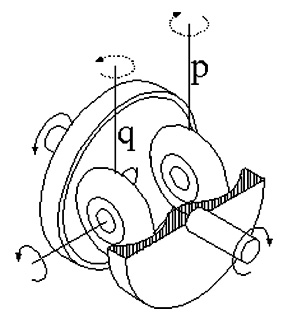
\includegraphics[height=165pt]{figure1.jpg}
\newline
\figurename{1~双滚子全环面CVT}
\end{figure}
\qquad\song\wuhao{许多研究人员试图提出一个模型,使锥盘和滚子之间的牵引系数能够准确计算。Jacod 等(2001)定义了一个数学模型:对于广泛范围的操作条件下预测等温椭圆形接触区的牵引系数。Newall和 Lee (2003) 提出了一种基于弹流润滑理论的模型,用来描述润滑油温度,压力与牵引油特性和牵引油粘度的关系。该模型能够计算牵引系数,滑移损失。Sanda 和 Hayakawa(2005) 通过假设在椭圆接触区内弹性、塑性、粘性三个因素相互独立,建立了一个简化模型。考虑过程中,弹性、塑性、粘性三者,只考虑占主导地位的其中之一。因此,无需通过粘弹塑模型得到数值解,便可以预测最大牵引力,并且预测的最大牵引系数误差在10\%之内。}

\qquad\song\wuhao{关于无级变速器动态分析及其效率计算的研究已经展开。Imanishi和Machida (2001)利用实验模型计算出半环面和全环面CVT的效率。Carbone等人(2004)进行动态分析比较了半环和全环形无级变速器的效率,建立了一个关于锥盘和滚子之间的理论弹流接触模型。为实现传动效率最大化,Delkhosh等人(2011)优化了半环面CVT,并其结果表明,其效率最高值出现在油温较低和输入锥盘转速较低时。}

\qquad\song\wuhao{CVT传动的效率、可控性、尺寸及重量等问题常常得到学者们的关注。研究发现,传统CVT往往存在效率低、难于控制的问题,而且跟手动变速器相比,传统CVT的体积更大,重量也更重。然而,关于全环面CVT的动力学和几何学优化问题的研究目前鲜有。本文将通过粒子群优化算法,试图使CVT传动效率最大化,能源损失最小化。}

\section{全环面CVT的动态分析}
\vspace*{-5pt}
\qquad\song\wuhao{为了开展优化分析,必须先建立与运动学和动力学参数相关的动力传动系统的效率模型。图2是全环面CVT示意图。}

\qquad\song\wuhao{R22和R0分别是滚子和锥盘的曲率半径。γ为滚子的旋转角度(顺时针方向)。R1和R3分别是输入、输出锥盘转轴与接触点之间的距离。}

\begin{figure}[H]
\centering%左对齐,flushright右对齐,centering,居中
  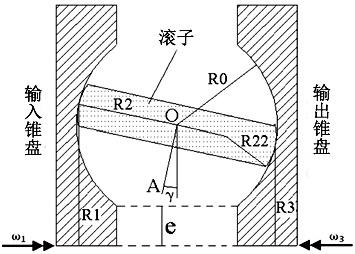
\includegraphics[height=165pt]{图二.jpg}
\newline
\figurename{2~全环面CVT示意图}
\end{figure}
\qquad\song\wuhao{当输入锥盘旋转,迫使滚轮绕轴OA转动,同样的转动传递给输出锥盘。滚子绕垂直于草图平面且通过O点的轴旋转,滚子倾角γ变化导致速比发生改变。由于γ可连续变化的,传动比也可连续变化。}

\qquad\song\wuhao{扭矩通过油膜剪切应力在锥盘和滚子之间传递。油膜剪应力与锥盘和滚子在接触点的线速度之差呈线性关系,也就是说锥盘和滚子之间一定存在滑移。无量纲滑移系数可由方程(1)和(2)表示出来:}
%\begin{equation}
%$\left\afrac{\RM{d}\sigma}{\RM{d}{Omega}\right|_{\RM{cm}}=\afrac{1}{4}$
%$$\mbox{\left\afrac{\RM{d}\sigma}{\RM{d}{Omega}\right|_{\RM{cm}}=\afrac{1}{4}}$$
%\begin{align}%写公式用align不要用equation,出不了。目前先用着。你可以看看为什么出不来,我暑假再看。
%$$\mbox{对任意的$x>0$}, \mbox{有 }f(x)>0. $$
%f(x_1,x_x,\ldots,x_n) = x_1^2 + x_2^2 + \cdots + x_n^2 
%&\afrac{r_{1}\omega_{1}}{2}
%-r_{2}\omega_{2}}{r_{1}\omega_{1}}
%\end{align}
%$$X_(
%\begin{align}
%S_{Pin} &=\afrac{1}{2}
%\end{align}
%\newenvironment{rcase}
 %   {\left.\begin{aligned}}
  %  {\end{aligned}\right\rbrace}
\iffalse
\begin{equation*}
  \begin{rcase}
    B' &= -\partial\times E          \\
    E' &=  \partial\times B - 4\pi j \,
  \end{rcase}
  \quad \text {Maxwell's equations},
%\end{equation*}
%\begin{equation*}
\end{equation*}
\fi
\iffalse
\flushleft
%\begin{equation}
%这是为了公式左对齐,一般latex默认居中对齐,我这里的方法不是最好。但是就是能用。如果急着用先用着。以后再找好方法更新。这只能对齐一个公式所以要重复地用
\begin{flalign}
\begin{split}
S_{Pin} =\frac{r_{1}\omega_{1}-r_{2}\omega_{2}}{r_{1}\omega_{1}}
\end{split}
\end{flalign}
\fi
\begin{align}
S_{Pin} =\frac{r_{1}\omega_{1}-r_{2}\omega_{2}}{r_{1}\omega_{1}}\\
S_{Pout} =\frac{r_{2}\omega_{2}-r_{3}\omega_{3}}{r_{2}\omega_{2}}
\end{align}
\qquad\song\wuhao{$\omega_{1}$和$\omega_{3}$分别表示输入锥盘和输出锥盘的转速。$\omega_{2}$表示滚子的转速。$r_{1}$和$r_{3}$用$\gamma$表示,如方程(3)和(4):}
\begin{align}
r_{1} = r_{0}(\mbox{\it{1}}+k+sin\gamma)\\
r_{3} = r_{0}(\mbox{\it{1}}+k-sin\gamma)
\end{align}
\qquad\song\wuhao{方程中,k是无量纲系数,定义为e与$r_{0}$的比值即\mbox{$\frac{e}{r_{0}}$}~\text{。}\\
则实际速比可得:}
\begin{align}
S_{r} = \frac{\omega_{3}}{\omega_{1}} = (\mbox{\it{1}}-S_{Pin})(\mbox{\it{1}}-S_{Pout})\frac{r_{1}}{r_{3}} = (\mbox{\it{1}}-S_{P})\frac{r_{1}}{r_{3}}
\end{align}
\qquad\song\wuhao{由于滑移系数的值较小,所以它们的乘积也很小,可以忽略。因此,方程中$S_{P}$等于$S_{Pin}$和$S_{Pout}$的和。理想的情况下,锥盘与滚子之间是没有滑动的。因此,理想情况下的速比为$S_{rlD}=\frac{r_{1}}{r_{3}}$ 。}
\begin{figure}[H]
\centering%左对齐,flushright右对齐,centering,居中
  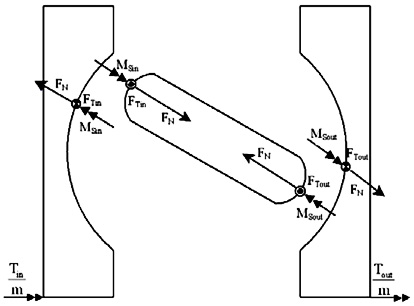
\includegraphics[height=165pt]{图三.jpg}
\newline
\figurename{3~全环面CVT的分离体受力分析图}
\end{figure}
\qquad\song\wuhao{因此,根据Carbone等人的研究,可以得到速度效率为:}
\begin{align}
\eta_{speed} = \frac{S_{r}}{S_{rlD}} =\mbox{\it{1}}-S_{p}
\end{align}
\qquad\song\wuhao{$S_{P}$为滑移系数。方程(6)表示锥盘和滚子之间由于打滑引起速度效率的下降。

~~~~图3为全环面CVT分离体受力分析图。Carbone等人(2004)对该系统进行动力学分析:}
\begin{align}
F_{Tin} = \mu_{in}F_{N}\\
F_{Tout} = \mu_{out}F_{N}
\end{align}
\qquad\song\wuhao{其中Fn是接触点正压力,Ftout是牵引力,它将输入扭矩分别传给输出盘和滚子。牵引力由接触区油膜的剪切应力产生。

~~~~由方程(7)和(8)可知,欲增大牵引力,唯有增大接触面正压力,或者选用较大牵引系数的牵引油。但由于接触表面的屈服应力限制了接触表面法向载荷的增加,因此,采用大牵引系数的牵引油才是提高牵引力的可行途径。

~~~~锥盘与滚子之间的自旋矩$M_{S_{in}}$和$M_{S_{out}}$表示为:}
\begin{align}
M_{S_{in}} = \chi_{in}F_{N}r_{1}\\
M_{S_{out}} = \chi_{out}F_{N}r_{3}
\end{align}
\qquad\song\wuhao{自旋距引起自旋损失,使传动效率降低。故输入牵引系数锡和输出牵引系数表示为:}
\begin{align}
t_{in} = \frac{T_{in}}{mnF_{N}r_{1}}\\
t_{out} = \frac{T_{out}}{mnF_{N}r_{3}}\\
t_{in}=\mu_{in}+\chi_{in}cos\gamma\\
t_{in}=\mu_{in}-\chi_{in}cos\gamma
\end{align}
\qquad\song\wuhao{$T_{in}$, $T_{out}$, n 和 m分别表示输入转矩,输出扭矩,滚子数和锥盘数。$\chi_{in}$, $\chi_{out}$为自旋动量系数,$\mu_{in}$ 和 $\mu_{out}$是牵引系数($F_{T}$和$F_{N}$之间的有效摩擦系数)。

~~~~则CVT的传动效率可通过(15)计算:}
\begin{align}
\eta = \frac{P_{out}}{P_{in}} = \frac{r_{1}T_{out}}{r_{3}T_{in}}\frac{r_{3}\omega_{3}}{r_{1}\omega_{1}} = \frac{t_{out}}{t_{in}}(\mbox{\it{1}}-S_{P})
\end{align}
\qquad\song\wuhao{从方程(13),(14)和(15)可看出自旋和滑动损失都会减少传动效率。但是,自旋损失对速度效率没有影响。同时,滑移不影响输出扭矩。由于自旋和滑移产生的功率损耗,可使用(16)和(17)计算:}
\begin{align}
SpinLoss = (M_{S_{in}}\omega_{S_{Pin}}+M_{S_{out}}\omega_{S_{Pout}})n\\
SlipLoss = (\mu_{in}S_{Pin}r_{1}\omega_{1}+\mu_{out}S_{Pout}r_{3}\omega{3})nF_{N}
\end{align}
\qquad\song\wuhao{$\omega_{S_{pin}}$和$\omega_{S_{pout}}$旋转速度可由式(18) 和(19)表示:}
\begin{align}
\omega_{S_{pin}} = \mid\omega_{1_{n}}-\omega_{2_{n}}\mid = \mid\omega_{1}cos\gamma\mid\\
\omega_{S_{pout}} = \mid\omega_{3_{n}}-\omega_{2_{n}}\mid = \mid\omega_{3}cos\gamma\mid
\end{align}
\section{接触模型}
\qquad\song\wuhao{进行优化过程需要建立基于几何和动态参数的研究,以牵引油特性作为输入的数值计算模型,该模型能够计算自旋角动量和牵引系数。由Jacod等人(2001)、Carbone等人(2004)、Szeri(2010)提出的模型适用于仿真弹流接触。该模型不考虑温度和压力对牵引油粘度的影响,以赫兹干摩擦理论描述压力分布。而在我们提出的模型中,考虑了温度和压力对牵引油粘度的影响(Yasutomi等人,1984)和最大剪应力(Newall和Lee,2003)的影响。(优化过程需要建立数值计算模型,模型利用几何和动态参数,将牵引油特性作为输入,能够计算的自旋角动量、牵引系数。该模型(Jacod等人,2001;Carbone等人,2004;Szeri,2010)用于仿真弹流接触。该模型中,用赫兹干摩擦理论描述压力分布。但温度和压力对牵引油粘度的影响并未考虑。在我们的模型中,温度和压力对牵引油粘度的影响(Yasutomi等人,1984)和最大剪应力(Newall和Lee,2003)被纳入考虑因素。)因此,方程(20),(21)和(22)表示了在P<1.2GPA下,牵引油,粘度,压力和温度四者之间的关系。}
\begin{table}[H]
\centering\caption{\label{tab:test}优化过程约束条件} %{|c|c|}是做有竖线的表
\begin{tabular}{lcl}
\hline
~~~~$\sigma_{eq}(Gpa)~~~~$~~~~~~ & $\leq1.2$~~~~~~~\\
~~~~$\mu_{in}$,$\mu_{out}~~~~$~~~~& ~$\le1.8$~~~~~~~~\\
\hline
\end{tabular}
\end{table}

\begin{thebibliography}{4}
\bibitem{1}Attia,N.A.,Datong,Q.I.N,Wankai,S.and Huaying,.L.I.(2003).A parametric study on the contact stress of half toroidal continuously variable transmission. J. Chongqing University 2,2,6-11.
\bibitem{2}Birch,S.(2000).Audi takes CVT from 15th century to 21st century. Automotive Engineering Int.,68-71.
\bibitem{3}Carbone, G.,Mangialardi,L. and Mantriota,G.(2001).Fuel Consumption of a Mid Class ehicle with Infinitely Variable Transmission. SAE. Warrendale.
\bibitem{4}Carbone, G.,Mangialardi,L. and Mantriota,G. (2004).A comparison of the performances of full and half toroidal traction drives. Mechanism and Machine Theory 39,9,921-942.
\bibitem{5}Delkhosh, M.,Saadat Foumani,M.,Boroushaki,M.,Ekhtiari,M.and Dehghani,M.(2011).Geometrical optimization of half toroidal CVT using particle swarm optimization. Scientia Iranica 18, 5, 1126−1132.
\bibitem{6}Dowson, D., Taylor, C. M. and Godet, M. (1991). Vehicle tribology. Proc. 17th Leeds-Lyon Symp. Tribology Held at the Institute of Tribology, Leeds University, Leeds,UK, 4th-7th September 1990, Elsevier Science Ltd.,18.
\bibitem{7}Imanishi,T.and Machida,H.(2001).Development of powertoros unit half-toroidal CVT (2).Motion \&Control,NSK Technical J.,10,1-8.
\bibitem{8}Jacod, B.,Venner,C. H.and Lugt,P. M.(2001).A generalized traction curve for EHL contacts. J.Tribology,123,248.
\bibitem{9}Machida,M. and Murakami,Y.(2000).Development of the half toroidal CVT powertors unit.NSK Tech. J. 9,669,15-26.
\bibitem{10}Nanbu, T.,Yasuda,Y., Ushijima,K.,Watanabe,J. and Zhu,D.(2008).Increase of traction coefficient due to surface microtexture. Tribology Letters 29,2,105-118.
\bibitem{11}Newall,J. and Lee,A. (2003).Measurement and prediction of spin losses in the EHL point contacts of the full toroidal variator. Tribology and Interface Engineering Series,43,769-779.
\bibitem{12}Park,N. G.,Ryu,J. H.,Lee, H. W.,Jeon, Y.H. and Zhang,N. (2009).Development of the inner spherical CVT for a motorcycle. Int. J. Automotive Technology 10,3,341-346.
\bibitem{13}Poon,S. Y. and Haines,D. J. (1966).Frictional behavior of lubricated rolling-contact elements. ARCHIVE,Proc.Institution of Mechanical Engineers 1847-1982 (vols 1-196),181,1966,363-389.
\bibitem{14}Rousseau,A.,Saglini,S.,Jaklov, M.,Gray,D. and Hardy,K.(2003).Trade-offs betweem fuel economy and Nox emssions using fuzzy logic control with a hybrid CVT configuration. Int. J. Automotive Technology 4,1,47-55.
\end{thebibliography}


%\qquad\song\wuhao{\mbox{$\omega_{1}$}啊啊啊$\omega_{1}$}% 两种表达都可以
%\end{equation}
$D^\prime_M\neq M^\prime_C(D)$
$\frac{r_{1}\omega_{1}-r_{2}\omega_{2}}{r_{1}\omega_{1}}$
$a_{1}$ \qquad $x^{2}$\qquad
$e^{-\alpha t}$ \qquad
$a^{3}_{ij}$
$e^{x^2} \neq {e^x}^2$
\newpage
$c^{2}=a^{2}+b^{2}$\\
$\lim_{n \to \infty}
\sum_{k=1}^n \frac{1}{k^2}
=\frac{pi^2}{6}$\\
\#\$\%\^ \& \_ \{\}\~\\
$a_{1}$ \qquad $x^{2}$\qquad
$e^{-\alpha t}$ \qquad
$a^{3}_{ij}$
$e^{x^2} \neq {e^x}^2$\\
$\sqrt{x}$ \qquad
$\sqrt{ x^{2}+\sqrt{y} }$
\qquad $\sqrt[3]{2}$[3pt]
$\surd[x^2 + y^2]$\\
$\overline{m+n}$ \qquad
$\underline{m+n}$\\
$\underbrace{ a+b+cdots+z }_{26}$\\
$\frac{ x^{2} }{ k+1 }\qquad
x^{ \frac{2}{k+1} }\qquad$










\end{multicols}



\end{document}






